\chapter{Concurrent Rules}

\section{Motivation}

What kind of concurrent rule do we expect and why?

Used in ~\cite{BezerraWEIT2016} and implemented in ~\cite{BezerraETMF2016}

\textbf{From the paper}

Given its formalism, there are several analysis techniques that can be performed over a Graph Grammar, including the \emph{concurrent rule} construction, which can be used to summarize the application of a sequence of several rules in one single step.

Graph Grammars that represent real systems usually have a considerable number of rules, possibly making it difficult to the modeller to foresee all possible rule interactions. Therefore it is important to have analysis techniques to address this issue, as well as tools that implement them.

We said earlier that the aim of calculating the concurrent rules is to summarize the combined effects of applying the transformations induced by a sequence of graph rules. Here we present how this can be done.

A \emph{rule sequence} is a list containing rules of a grammar in an specific order in which the modeller wants them to be applied. Given a rule sequence \mbox{$r =$ \rulesequence}, the construction of its correspondents concurrent rules is done by recursively combining pairs of subsequent rules, where the pairwise combination is defined as follows~\cite{Ehrig2006,Lambers2010}:  

\section{Concurrent Rules}

\begin{definition}{Concurrent Rules}

\diagram{
  L_c\ar[d]\ar\ar@{}[dr]|{(3)} & K_c\ar[d]\ar[l]\ar[r] \ar@{}[dr]|{(1)} & R_c\ar[dr]^{e_1} & & L_n\ar[dl]_{e_2} & K_n\ar[d]\ar[l]\ar[r]\ar@{}[dl]|{(2)} & R_n\ar[d]\ar@{}[dl]|{(4)}\\
  L & C_c\ar[l]^{c_l}\ar[rr]_{c_r} & & \textit{E} & & C_n\ar[ll]^{n_l}\ar[r]_{n_r} & R\\
  & & & K\ar@{.>}@/1pc/[llu]^{k_c}\ar@{.>}@/1pc/[urr]_{k_n}\ar@{}[u]|{(5)} & & &
}
\end{definition}

\begin{definition}{Downward Shifted NACs}

\diagram{
  N'_j\ar@{.>}@/0.5pc/[r]^{e_{ji}} & N_i\ar@{}[dl]|{=}\\
  A\ar[r]_{m}\ar[u]^{n'_j} & B\ar[u]_{n_i}
}

For each $NAC(n'_j)$ on $A$ with $n'_j : A \rightarrow N'_j$ and $m : A \rightarrow B$, 
let $D_m(NAC(n'_j)) = \{ NAC(n_i)|i \in I, n_i : B \rightarrow N_i \}$ where $I$ and $n_i$ 
are constructed as follows:
\begin{itemize}
  \item $i \in I$ iff $(e_{ji}, n_i)$ with $e_{ji} : N'_j \rightarrow N_i$ jointly surjective 
  \item $e_{ji} \circ n_i = n_i \circ m$
  \item $e_{ji}$ injective
\end{itemize}

For each set of NACs $NAC_A = {NAC(N_j)| j \in J}$ on $A$ the downward shift of $NAC_A$ is then defined as: $D_m(NAC_A) = \cup_{j \in J}D_m(NAC(n'_j))$. $D_m$ is also called the \emph{Downward shift of $NAC_A$}.

\end{definition}

\begin{definition}{Left NACs from Right NACs}

\centerline{\xymatrix{
  L\ar[d]_{n'_i} & K\ar[l]\ar[r]\ar[d] & R\ar[d]^{n_i}\\
  N'_i\ar@{}[ur]|{(2)} & D\ar[l]\ar[r] & N_i\ar@{}[ul]|{(1)}
}}

\end{definition}

\begin{definition}{Concurrent Rules with NACs}

A concurrent rule is
\end{definition}

\centerline{
\xymatrix{
  N_i & & & & N_j & & \\
  L_c\ar[d]\ar[u]^{n_i}\ar@{}[dr]|{(3)} & K_c\ar[d]\ar[l]\ar[r] \ar@{}[dr]|{(1)} & R_c\ar[dr]^{e_1} & & L_n\ar[dl]_{e_2}\ar[u]^{n_j} & K_n\ar[d]\ar[l]\ar[r]\ar@{}[dl]|{(2)} & R_n\ar[d]\ar@{}[dl]|{(4)}\\
  L & C_c\ar[l]^{c_l}\ar[rr]_{c_r} & & \textit{E} & & C_n\ar[ll]^{n_l}\ar[r]_{n_r} & R\\
  & & & K\ar@{.>}@/1pc/[llu]^{k_c}\ar@{.>}@/1pc/[urr]_{k_n}\ar@{}[u]|{(5)} & & &
}}

\begin{itemize}
\item $n = 0$ The \emph{concurrent rule} $p_c$ with NACs for rule $p_0$ with NACs is $p_0$ with NACs itself.
\item $n \geqslant 1$ A concurrent rule $p_c = p'_c \ast_E p_n $ with NACs for the rule sequence \rulesequence is defined recursively as $p_c = (l_c \circ k_c : K \rightarrow L, r_n \circ k_n : K \rightarrow R)$ where 
  \begin{itemize}
  \item $p'_c : L'_c \leftarrow K'_c \rightarrow R'_c$ is a concurrent rule for the sequence $p_0,\ldots,p_{n-1}$
  \item $(e'_c,e_n)$ is jointly surjective
  \item (1), (2), (3) and (4) are pushouts
  \item (5) is a pullback
  \item $N_i$ is shifted over morphism $l'$
  \item $N_j$ is shifted over morphism $e_2$ and then over the ``rule'' $q'_c = l_c : C_c \rightarrow L, r_c : C_c \rightarrow E$
  \end{itemize}
\end{itemize}

\begin{definition}{Concurrent Rules induced by Dependencies}

  \textbf{incomplete}

  The default algorithm constructs the concurrent rules based on all the overlappings of the right side of the first rule and left side of the second rule, allowing us to see how the elements created/preserved by one rule can be connected with the elements deleted/preserved by the other.

  One way to restrict the number of possible concurrent rules and still generate meaningful rules is to filter and use only the overlappings associated with dependencies~\cite{Lambers2006} between subsequent pairs of rules. The idea behind this is to use only the overlappings where (1) the elements needed for the second rule to be applied are explicitly created by the first one or (2) the elements forbidden by the NACs of the second rule are explicitly deleted by the first.

  For the first case, we only need to filter the overlappings in the concurrent rule diagram where $\nexists h_{12} : R'_c \rightarrow C_n$ such that $(l_n \circ h_{12} = e_1$ and $r_n \circ h_{12} \models N^{-1}_i)$ or $\nexists h_{21} : L_n \rightarrow C_c$ such that $(r_c \circ h_{21} = e_2$ and $l_c \circ h_{21} \models N_j)$.

  However, this notion does not take into consideration the elements whose existence is forbidden by the NACs of the second rule and would then forbid its application, but once deleted by the first rule the application of the second is enabled.

  We did not find on the literature a construction to capture those cases, however an adaptation of the concurrent rule algorithm can be made based on the algorithm for calculating dependencies between the rules defined in~\cite{Lambers2006}. Besides the overlappings between $(R'_c, L_n)$ that represent dependencies, we generate \emph{also} the overlappings of the left side of the first rule $L'_c$ with the NACs $N_j$ and check whether the rewritings are possible, in which case the
  diagram for the corresponding concurrent rule construction can be seen as follows:

\diagram{
  N_i& & & & N_j\ar@{.>}@/_3pc/[ddllll]_{e_2} & & \\
  L_c\ar[u]^{n_i}\ar[d]_{e_1}\ar@{}[dr]|{(1)} & K_c\ar[d]\ar[l]\ar[r] \ar@{}[dr]|{(2)} & R_c\ar[dr]^{m'_1} & & L_n\ar[dl]_{m_2}\ar[u]^{n_j} & K_n\ar[d]\ar[l]\ar[r]\ar@{}[dl]|{(3)} & R_n\ar[d]^{m'_2}\ar@{}[dl]|{(4)}\\
  \textit{E} & C_c\ar[l]|{c_l}\ar[rr]|{c_r} & & P_1 & & C_n\ar[ll]|{n_l}\ar[r]|{n_r} & P_2\\
  & & & K\ar@{.>}@/1pc/[llu]|{k_c}\ar@{.>}@/1pc/[urr]|{k_n}\ar@{}[u]|{(5)} & & & 
}

\end{definition}
% \ar@{.>}@/_1pc/[dlll]|{X_{h_{21}}}

\begin{thm}{EpiPairs}
  \begin{proof}{Incomplete}
  \end{proof}
\end{thm}

\section{Dealing with the combinatorial explosion}\label{sec:explosion}

There exist some strategies that can help dealing with the combinatorial explosion of by addressing some specificities of the problem domain. The strategies explained in the following do not solve the theoretical worst cases, but they have been showed to be good enough in most of our practical cases.

\subsection{Trivially-triggered NACs}

For each pair of rules $(p_c,p_n)$ for which we want to generate the corresponding concurrent rules, we must first generate all possible overlappings between $R_c$ and $L_n$, check whether they satisfy the gluing conditions and calculate the pushouts and pullbacks that will result in the concurrent rules. However, it is possible that some of the generated overlappings result in epimorphic pairs $(E, e_1 : R_c \rightarrow E, e_2 : L_n \rightarrow E)$ whose morphisms $e_1$ or $e_2$ do not satisfy
the right NACs of $p_c$ or the left NACs of $p_n$, respectively.

In such cases, the NACs forbid the existence of valid transformations \mbox{$L \xRightarrow{p_c,l'} E$} and $E \xRightarrow{p_n,r'} R$ even though the gluing conditions are satisfied. It means that the rules could not be applied over the graph $E$. We may them ignore such overlappings when calculating possible concurrent rules.

If we do maintain those pairs for computation, as the shift of NACs aims to translate the NACs of each rule to sets of equivalent NACs in the concurrent rules, we would generate rules where for every possible match of $L$, there will always be a NAC not satisfied by $m$, thus the rule would never be applicable.

\subsection{Graph Constraints}\label{sec:constraints}

Graph constraints can be used to globally enforce or prohibit the existence of certain structures in the graphs that can be generated by a graph grammar. For example, they can be used to define minimal and maximal multiplicities for nodes and edges.

When calculating the concurrent rules for a pair $(p_c, p_n)$ we first use them similarly to the use of NACs, checking whether the generated overlappings satisfy the graph constraints, cutting off those who do not, which can also lead to a reduction of possible concurrent rules. Fig~\ref{fig:constraints} shows two negative atomic constraints that (a) forbid the existence of more than one server and (b) forbid a piece of data of being in two different messages at the same time. Look at
Fig~\ref{fig:epipairs} again to see that two of the overlappings would be cut off by these constraints.

We can still use the graph constraints to cut off even more concurrent rule candidates, because even though the overlappings satisfy the gluing conditions and NACs, the resulting $lhs$ and $rhs$ may still not satisfy the graph constraints. 

When dealing with injective morphisms, if a graph $L$ of a rule does not satisfy the graph constraints, no possible \match{} can be found in which $G$ satisfies the constraints, thus the rule can never be applied and we can discard it. Similar reasoning can be applied to the $R$ graph and \comatch{}.

\begin{figure}
\centering
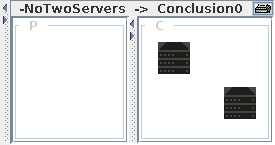
\includegraphics{grammar/no_two_servers}
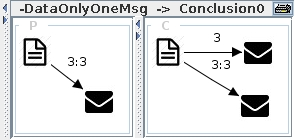
\includegraphics{grammar/data_no_two_msgs}
\caption{\label{fig:constraints} Negative atomic constraints for server}
\end{figure}

\subsection{Concurrent Rules Induced by Dependencies}

The default algorithm constructs the concurrent rules based on all the overlappings of the right side of the first rule and left side of the second rule, allowing us to see how the elements created/preserved by one rule can be connected with the elements deleted/preserved by the other.

One way to restrict the number of possible concurrent rules and still generate meaningful rules is to filter and use only the overlappings associated with dependencies~\cite{Lambers2006} between subsequent pairs of rules. The idea behind this is to use only the overlappings where (1) the elements needed for the second rule to be applied are explicitly created by the first one or (2) the elements forbidden by the NACs of the second rule are explicitly deleted by the first.

For the first case, we only need to filter the overlappings in the concurrent rule diagram where $\nexists h_{12} : R'_c \rightarrow C_n$ such that $(l_n \circ h_{12} = e_1$ and $r_n \circ h_{12} \models N^{-1}_i)$ or $\nexists h_{21} : L_n \rightarrow C_c$ such that $(r_c \circ h_{21} = e_2$ and $l_c \circ h_{21} \models N_j)$.

However, this notion does not take into consideration the elements whose existence is forbidden by the NACs of the second rule and would then forbid its application, but once deleted by the first rule the application of the second is enabled.

We did not find on the literature a construction to capture those cases, however an adaptation of the concurrent rule algorithm can be made based on the algorithm for calculating dependencies between the rules defined in~\cite{Lambers2006}. Besides the overlappings between $(R'_c, L_n)$ that represent dependencies, we generate \emph{also} the overlappings of the left side of the first rule $L'_c$ with the NACs $N_j$ and check whether the rewritings are possible, in which case the
diagram for the corresponding concurrent rule construction can be seen as follows:

\diagram{
    N_i& & & & N_j\ar@{.>}@/_3pc/[ddllll]_{e_2} & & \\
      L'_c\ar[u]^{n_i}\ar[d]_{e_1}\ar@{}[dr]|{(1)} & K'_c\ar[d]\ar[l]\ar[r] \ar@{}[dr]|{(2)} & R'_c\ar[dr]^{m'_1} & & L_n\ar[dl]_{m_2}\ar[u]^{n_j} & K_n\ar[d]\ar[l]\ar[r]\ar@{}[dl]|{(3)} & R_n\ar[d]^{m'_2}\ar@{}[dl]|{(4)}\\
        \textit{E} & C_c\ar[l]|{c_l}\ar[rr]|{c_r} & & P_1 & & C_n\ar[ll]|{n_l}\ar[r]|{n_r} & P_2\\
          & & & K\ar@{.>}@/1pc/[llu]|{k_c}\ar@{.>}@/1pc/[urr]|{k_n}\ar@{}[u]|{(5)} & & & 
          }\vspace{-15pt}


          \subsection{Maximal Concurrent Rule}

          Sometimes, instead of generating all possible overlappings or even all the dependencies, the modeller is interested in seeing only the maximal interactions between the elements of each rule in the sequence, thus we may filter the overlappings with the least number of elements, capturing the cases where the elements of each rule are as connected as possible. Note that the rule in Fig~\ref{fig:concurrent_rule_construction} is a maximal concurrent rule.

\subsection{Inapplicable concurrent rules}

\begin{definition}{Rules with trivially triggered NACs}
\end{definition}

\begin{thm}{Propagation of trivially triggered NACs over concurrent rules}
  \begin{proof}{Yet to come}
  \end{proof}
\end{thm}

\begin{definition}{Breaking constraint rules}
\end{definition}

\section{Comparison or Results}
